\section{Experimental Evidence}
\label{sec:experiments}
We separate generated-model validation, solving frozen models and handling real data. Local benchmark and
synthetic-pipeline conditions use three repetitions; later backend comparisons also use three submissions per
condition. External repetitions are resubmissions without exposed hardware RNG seeds. Their search times are
not equivalent compute resources. No failed experiment is replaced by a simulated hardware result.

\subsection{Synthetic end-to-end modelling}
For twelve categories, we supplied one realistic request and ran clarification and modelling three times,
answering questions with the proposed defaults. The instances came from the generated synthetic-data function,
so this suite tests the pipeline rather than autonomous acquisition. All 36 clarifications converged and all
36 models passed validation; 35 produced a validated figure. Median pipeline time was 5.6 minutes.

One GPU solve per category reached the exact optimum in seven of nine categories with known references.
A portfolio instance had no feasible GPU result, and network design remained far from optimal.
Two development checks were initially wrong: a sorting detector rejected models with overlapping constraints,
and visualization was skipped when enumeration was impossible. Both were corrected and affected categories
rerun. These results concern the resulting evaluation configuration, not a frozen first-attempt success rate.

Mechanism observations explain some local-model failures. On a 1,680-variable scheduling model with 3,324
constraints, describing ten constraint families reduced tuning prompts from approximately 53k--54k to 2k--3k
tokens. Splitting model generation from visualization produced an EV-charger model and figure in two of three
runs. A reasoning cap with one retry without reasoning reduced empty Coder answers from 7/240 (2.9\%) to
5/521 (1.0\%). These observations are narrower than a controlled estimate of the value of every agent role.

\subsection{Routing scale and limits}
An LLM-generated single-vehicle routing model uses $n^2$ position variables. With ten-second CGA jobs, all
returned tours were feasible up to 60 stops (3,600 variables). Quality was exact up to ten stops and matched a
20-restart 2-opt reference up to 30 stops. Relative differences rose to 12.4\%, 27.2\% and 43.5\% at 40, 50 and
60 stops. The references are exact only at small sizes; larger references are feasible heuristics.
These are one-shot size measurements, not repeated evidence of an annealing advantage.

\subsection{Frozen-model backend comparisons}
The red-wine, 60-item knapsack and 80-item conflict-selection models were frozen before comparing defaults,
TPE penalty search and an LLM tuning agent. Each condition allowed at most three calls. SA used 60 reads and
300 sweeps; CGA used a three-second search limit. All 54 SA/CGA conditions produced feasible solutions.
The same three models and policies produced feasible results in all 27 Leap Hybrid conditions, using 72 actual
submissions. Every Hybrid call explicitly requested ten seconds; instances requiring a larger service minimum
were refused rather than assigned a longer time. Figure~\ref{fig:evidence} reports the observed mean gaps.

\begin{figure*}[t]
\centering
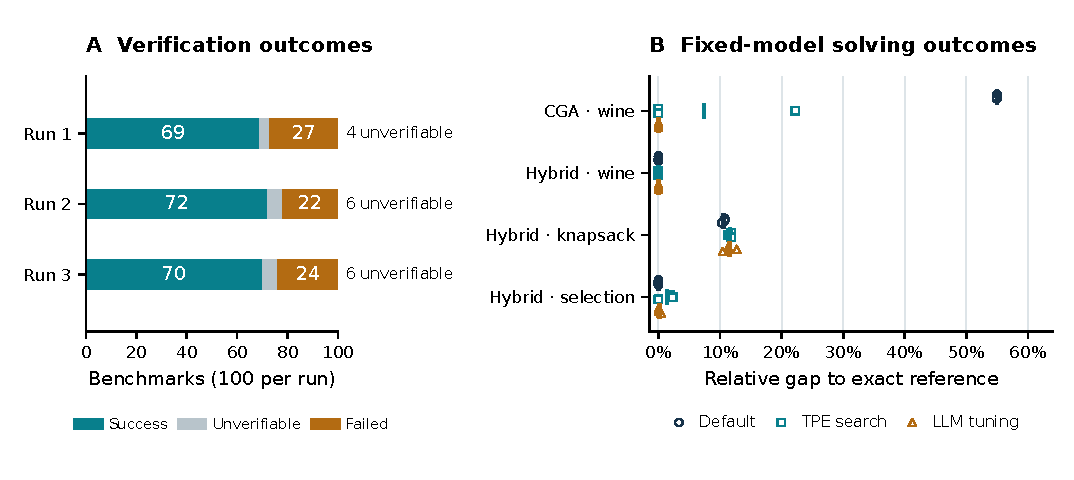
\includegraphics[width=\textwidth]{figures/evidence.pdf}
\caption{Recorded evaluation outcomes. Left: successes and unverifiable cases across three runs on the same
100 benchmarks; the remaining cases failed verification. Right: mean original-objective gaps on four selected
frozen-model/backend combinations, three repetitions per policy. Hollow markers show all three observed repetitions per condition; short vertical marks show their means. No confidence intervals are inferred.
CGA and Hybrid have different per-call limits; the plot does not establish a hardware advantage.}
\label{fig:evidence}
\end{figure*}


CGA defaults reached the reference on both non-wine models. On wine, mean gaps were 0.5495 for defaults,
0.0740 for TPE and 0.0000 for LLM tuning. Hybrid attained the wine reference under all three policies, but
knapsack mean gaps remained 0.1060, 0.1164 and 0.1149. These outcomes vary with model and backend.
Hybrid is not direct-QPU sampling, and its ten-second ceiling differs from CGA's three-second ceiling.
A real DA submission was rejected at the monthly account limit; no successful DA results are reported.

\subsection{Penalty search as a supporting component}
An earlier budget-matched SA comparison used 80 paired runs per policy. LLM variants reached mean gaps of
0.073--0.078 versus 0.084 for defaults, but defaults attained the optimum more often (38/80 versus 25--35/80).
Splitting tuning into diagnosis and refinement did not help ($p=0.10$), nor did retrieval of tuning knowledge
($p=0.17$). These results do not evaluate modelling-pattern retrieval.

In a separate eight-instance comparison with ten seeds and eight policies (640 SA runs), all runs returned
feasible results. Default weights had the lowest mean gap, 0.0932; penalty-only TPE, grid, cross-entropy and
sequential search had means 0.1080, 0.1070, 0.1372 and 0.1003. Paired Wilcoxon tests on eight instance-averaged
differences gave Holm-adjusted $p=0.03125$ for each of the four comparisons. Runs allowed six calls with 60
reads and 300 sweeps per call. This negative result supports keeping penalty search subordinate to data and
model validation, rather than claiming a generally superior tuning strategy.

\subsection{Real data: preparation and specified-source pilots}
The preprocessing toolkit reproduced Taipei's published village population from 63,315 rows containing ROC
years, stacked months, gender categories and mixed administrative levels, then joined official boundaries in
TWD97 coordinates. The cleaned total of 2,418,872 matched the published city total. Of 456 villages, 455 matched
by name; the final one required a variant-character match. An earlier transformation retained a city-total row
and doubled population, which aggregate provenance checks exposed. This is a toolkit validation, not autonomous
end-to-end acceptance.

A specified-source wine pilot used all 1,599 UCI records\cite{uciWine}. The local LLM wrote the model and
Adapter; selecting five features achieved objective 0.7497088247 after four SA calls, matching enumeration of
all 2,048 assignments. The successful fresh run used approximately 64 seconds and 20,596 LLM tokens.
A recovered UCI wholesale-customer pilot\cite{uciWholesale} formed three equal groups from 24 sampled records,
with objective 856.8319 versus 1021.7818 for a feasible baseline (16.1\% lower).
A recovered karate-club case delivered two groups of 17 with 17 cut edges from the baseline because annealing
returned 22. These pilots used manually specified inputs or independent case-specific checks; some reused
models or caches. They do not establish unrestricted autonomous data acquisition or a prospective success rate.

\subsection{Autonomous acceptance protocol and remaining execution}
A new runner starts without saved models, instances or LLM cache. Agents receive a request and fixed user
answers specifying settings, without formulas or field names. Each configuration must find and download data.
Three tasks are defined: five Taipei charger sites maximizing population covered within one kilometre;
a tour of all YouBike stations within 500 metres of a specified point; and three equal-size groups of eligible
AED inspection locations. The charger task preserves all villages and prohibits sampling.

An external case-specific judge uses frozen raw-data truth withheld from the runtime agents. It checks
one-to-one entity coverage, coordinates and measured values; tests model feasibility and objective ranking on
30 sampled decisions; and verifies delivered requirements and quality within 10\% of a feasible reference where
available. The ranking threshold is 0.9. Data correctness, model correctness and usable delivery are separate
outcomes; joint success requires all three. Judge failures and unsupported representations are retained.

Five configurations compare a direct LLM, a structured workflow, added independent checkers, added cross-stage
repair and added modelling-pattern retrieval. Three repetitions on three tasks require 45 runs. An optional
comparison disables only clarification web lookup, giving 54 runs. Common ceilings include four model attempts,
three solver calls using CGA defaults and bounded repairs. The direct configuration has different acquisition
tools and download limits, so it compares complete systems rather than isolating agent count. Automated
confirmations are fixtures rather than observed user-effort measurements.

Existing development records span changing code and prompts and include both successful YouBike deliveries
and upstream failures. They are not pooled into a success rate. Code, prompts, cases and truth are hashed for
new frozen batches; the repeated comparison remains incomplete. Consequently, no end-to-end advantage for
multi-agent coordination, checking, repair or modelling retrieval is reported here.
